\documentclass{article} % For LaTeX2e
\usepackage{nips15submit_e,times}
\usepackage{hyperref}
\usepackage{url}
\usepackage{graphicx} 
\usepackage[T1]{fontenc}
\usepackage{bm}
\nipsfinalcopy % Uncomment for camera-ready version
%\documentstyle[nips14submit_09,times,art10]{article} % For LaTeX 2.09


\title{MAT 258A, Final Project\\
	\small Lasso Solvers: Quadratic Programming and LARS}


\author{Yilun Zhang\\
	999486337}

% The \author macro works with any number of authors. There are two commands
% used to separate the names and addresses of multiple authors: \And and \AND.
%
% Using \And between authors leaves it to \LaTeX{} to determine where to break
% the lines. Using \AND forces a linebreak at that point. So, if \LaTeX{}
% puts 3 of 4 authors names on the first line, and the last on the second
% line, try using \AND instead of \And before the third author name.

\newcommand{\fix}{\marginpar{FIX}}
\newcommand{\new}{\marginpar{NEW}}

%\nipsfinalcopy % Uncomment for camera-ready version

\begin{document}


\maketitle

\begin{abstract}
Lasso[1], proposed by Tibshirani in 1996, is short for least absolute shrinkage and selection operator.  It can estimate the regression coefficients and select them at the same time. But LASSO wasn't popular when it is invented. Because this method involves absolute constraint which is not derivable. Methods and computational power at that time can't solve lasso problem in a short time. In this project I will first show under modification, lasso can be rewritten into standard quadratic programming problem and then introduce the least angle regression method (LARS).

\end{abstract}

\section{The Lasso Problem\label{sec1}}

Robert Tibshirani's 1996 paper R[1], introduces the lasso which can do the parameter estimation and selection at the same time. It sacrifice a little bias but greatly reduced prediction error often occurs in ordinary least square estimator, retains nice properties of both ridge and subset selection. 

The most part of the paper introduces lasso based on a linear regression model. Suppose $(\bm{x}^i,y_i),\,i=1,2,\cdots,N$ are the data where $y$ has mean 0 and $\bm{x}$ is normalized such that $\sum_ix_{ij}/N=0$ and $\sum_ix^2_{ij}/N=1$. Different from OLS(ordinary least square), lasso estimator is obtained by minimizing
\begin{equation}
\hat{\bm{\beta}}=arg min \{\sum_{i=1}^{N}(y_i-\sum_j\beta_jx_{ij})^2\}\label{eq1}
\end{equation}
with constraint\begin{equation}
||\bm{\beta}||_1=\sum_j|\beta_j|\le t\label{eq2}
\end{equation}
$t$ is a prespecified parameter.
By Lagrange form, this is equivalent to minimizing
\begin{equation}
\hat{\bm{\beta}}=arg min \{\sum_{i=1}^{N}(y_i-\sum_j\beta_jx_{ij})^2+\lambda||\bm{\beta}||_1\}\label{eq3}
\end{equation}
This means put a $L_1$ penalty on the coefficients. The small $t$ or large $\lambda$ will cause many coefficient set to be 0 by the property of $L_1$ norm. This will do the predictor selection automatically. This will be benefit if we believe the underlying model has sparse representation.

\section{Quadratic Programming}
Many previous works (such as Busa J, 2012 [2]) proves a simple method that can rewrite lasso into a standard quadratic programming problem that no absolute operation involves.

Consider $$ \begin{array}{ll}
	minimize_\beta &||Y-X\bm{\beta}||_2^2\\
	subject\, to & ||\bm{\beta}||_1 < t
\end{array}
$$
this is equivalent to $$ \begin{array}{ll}
minimize_\beta &\frac{1}{2}\bm{\beta}^TH\bm{\beta}+f^T\bm{\beta}\\
subject\, to & ||\bm{\beta}||_1 < t
\end{array}
$$where $H=2X^TX$, $f=-2X^TY$. Then let \[
\beta_i=\beta_i^+-\beta^-_i
\] and\[
\beta_i^+=\frac{|\beta_i|+\beta_i}{2}\quad \beta_i^-=\frac{|\beta_i|-\beta_i}{2}
\]
obviously, $|\beta_i|=\beta_i^++\beta^-_i$. Then we have $$ \begin{array}{ll}
minimize_\beta &\frac{1}{2}(\bm{\beta}^+-\bm{\beta}^-)^TH(\bm{\beta}^+-\bm{\beta}^-)+f^T(\bm{\beta}^+-\bm{\beta}^-)\\
subject\, to & \sum_i[\beta_i^++\beta^-_i] < t, \, \beta_i^+,\,\beta^-_i\le0
\end{array}
$$
The objective function becomes
$$\frac{1}{2} \left[\begin{array}{l}
\bm{\beta}^+\\\bm{\beta}^-
\end{array}\right]^T\left[\begin{array}{ll}
H &-H\\
-H & H
\end{array}\right]\left[\begin{array}{l}
\bm{\beta}^+\\\bm{\beta}^-
\end{array}\right]+\left[f^T \,-f^T\right]\left[\begin{array}{l}
\bm{\beta}^+\\\bm{\beta}^-
\end{array}\right]
$$The constraint becomes
\[
\left[\begin{array}{l}
1_{2p}^T\\
-I_{2p}
\end{array}\right]\left[\begin{array}{l}
\bm{\beta}^+\\\bm{\beta}^-
\end{array}\right] \le \left[\begin{array}{l}
t\\
0_{2p}^T\end{array}\right]
\]where $1_{2p}$ is $2p$ by 1 vector with all 1, $I_{2p}$ is $2p\times2p$ identical matrix, $1_{2p}$ is $2p$ by 1 vector with all 0.

 Let\[
Q=\left[\begin{array}{ll}
H &-H\\
-H & H
\end{array}\right]\quad c^T=\left[f^T \,-f^T\right]\quad A=\left[\begin{array}{l}
1_{2p}^T\\
-I_{2p}
\end{array}\right] \quad\]
\[ b = \left[\begin{array}{l}
t\\
0_{2p}^T\end{array}\right]\quad x = \left[\begin{array}{l}
\bm{\beta}^+\\\bm{\beta}^-
\end{array}\right]
\] The lasso problem can be written as standard quadratic programming problem:$$ \begin{array}{ll}
minimize_x &\frac{1}{2}x^TQx+c^Tx\\
subject\, to & Ax\le b
\end{array}
$$

\section{The LARS Algorithm}
Efron et al [3] proposed the least angle regression algorithm. This algorithm is computationally efficient. It only need $p$ iterations for $p$ predictors.
\subsection{Notation}
Suppose $y$ is the response variable of interest. $x_1,x_2,\cdots x_p$ are observed predictor variables assumed to be linearly independent and nomalized as in section \ref{sec1}. $\mathcal{A}$ denotes a subset of index ($1,2,\cdots,p$), define the matrix $$X_\mathcal{A}=(\cdots,s_jx_j,\cdots)_{j\in\mathcal{A}}$$
\[
G_\mathcal{A}=X_\mathcal{A}'X_\mathcal{A} \, and \, A_\mathcal{A}=(1'_\mathcal{A}G^{-1}1_\mathcal{A})^{-1/2}.
\]
The equiangular vector $u_\mathcal{A}=X_\mathcal{A}w_\mathcal{A}$, where $w_\mathcal{A}=A_\mathcal{A}G^{-1}1_\mathcal{A}$.
\subsection{The LARS algorithm}
\begin{enumerate}
	\item Start with $\hat{\mu}_0=0$
	\item In each step, update $\mu_i$ in the following way:\\
	(1). Compute $\hat{c}=X'(y-\hat{\mu}_i)$
	(2). Let $\hat{C}=max_j{|\hat{c}_j|}$ and add $j$ into active set $\mathcal{A}$.
	(3). Set $s_j=sign(\hat{c}_j)$ for all $j$ in $\mathcal{A}$.
	(4). Compute $X_\mathcal{A},\,A_\mathcal{A},\,u_\mathcal{A}$ defined in the last section, and \[
	a=X'u_\mathcal{A}
	\]
	(5). Update \[
	\hat{\mu}_{i+1}=\hat{\mu}_i+\hat{\gamma}u_\mathcal{A}
	\]where\[
	\hat{\gamma}=\min^+_{j\in\mathcal{A}}\left\{\frac{\hat{C}-\hat{c}_j}{A_\mathcal{A}-a_j},\frac{\hat{C}+\hat{c}_j}{A_\mathcal{A}+a_j}\right\}
	\]
	\item Continue updating until $p$ step, or the max correlation is 0, or reaches bound.
\end{enumerate}

\subsection{Lasso Modification}
Efron et al [3] proves that under certain modification, the LARS solution is the lasso solution.

Let $\hat{d}$ be the $p\times1$ vector with $j$th entry equaling $s_jw_{\mathcal{A}j}$ and all other entries to be 0. Let \[
\gamma_j=-\hat{\beta}_j/\hat{d}_j.
\] and \[
\tilde{\gamma}=\min_{\gamma_j>0}(\gamma_j)
\]
The lasso modification is if $\tilde{\gamma}<\hat{\gamma}$, stop the ongoing step at $\gamma=\tilde{\gamma}$ and remove $\tilde{j}$ from the calculation of next equiangular direction. i.e,\[
\hat{\mu}_\mathcal{A}^+=\hat{\mu}_\mathcal{A}+\tilde{\gamma}u_\mathcal{A}
\]and\[
\mathcal{A}^+=\mathcal{A}-\tilde{j}
\]
\section{Code and Result}
The \emph{QPlasso.m} implements quadratic programming method with algorithm 'interior-point-convex'. The \emph{lars.m} (I referenced matlab package 'lar' and R packages 'lars', some piece of code are similar to the code in the package) is the matlab code implements LARS algorithm with lasso modification. The codes is available on \url{https://github.com/lunge111/MAT258A}.

The fitting result of these two method agrees with each other generally. One major difference is for those 0 coefficients, LARS will set them exactly equal to 0 but quadratic programming will yield some very small value. Table \ref{tab1} shows different value fitted by these two methods on diabetes data set (the data set used in [3]).

\begin{table}
	\centering
	\begin{tabular}{|l|c|c|}
		\hline
coeffcients &	quadratic programming & LARS\\
\hline	
$\beta_1$	&	-1.38714880002693e-19& 0\\
$\beta_2$	&	-3.00961394071294e-20&0\\
$\beta_3$	&	80.0607375117748&80.0607375117755\\
$\beta_4$	&	3.49816666282146e-18&0\\
$\beta_5$	&	-4.90071425713167e-19&0\\
$\beta_6$	&	-3.16049168444261e-20&0\\
$\beta_7$	&	-1.08009935664724e-18&0\\
$\beta_8$	&	7.05816673079248e-19&0\\
$\beta_9$	&	19.9392624882252& 19.9392624882245\\
$\beta_{10}$	&	2.00773278278871e-19&0\\
\hline
	\end{tabular}
	\caption{\label{tab1} Fitting the diabetes data set by LARS and quadratic programming  at $t=100$}
\end{table}

Both two methods are very fast. The LARS finishes 400 fitting in 1 second, while quadratic programming does it in 2 seconds, averagely 9 iterations are used.
\section{Reproduction of Paper Result}
I reproduced Figure 1 in [3]. The result agrees with the paper.
\begin{figure}
	\centering
	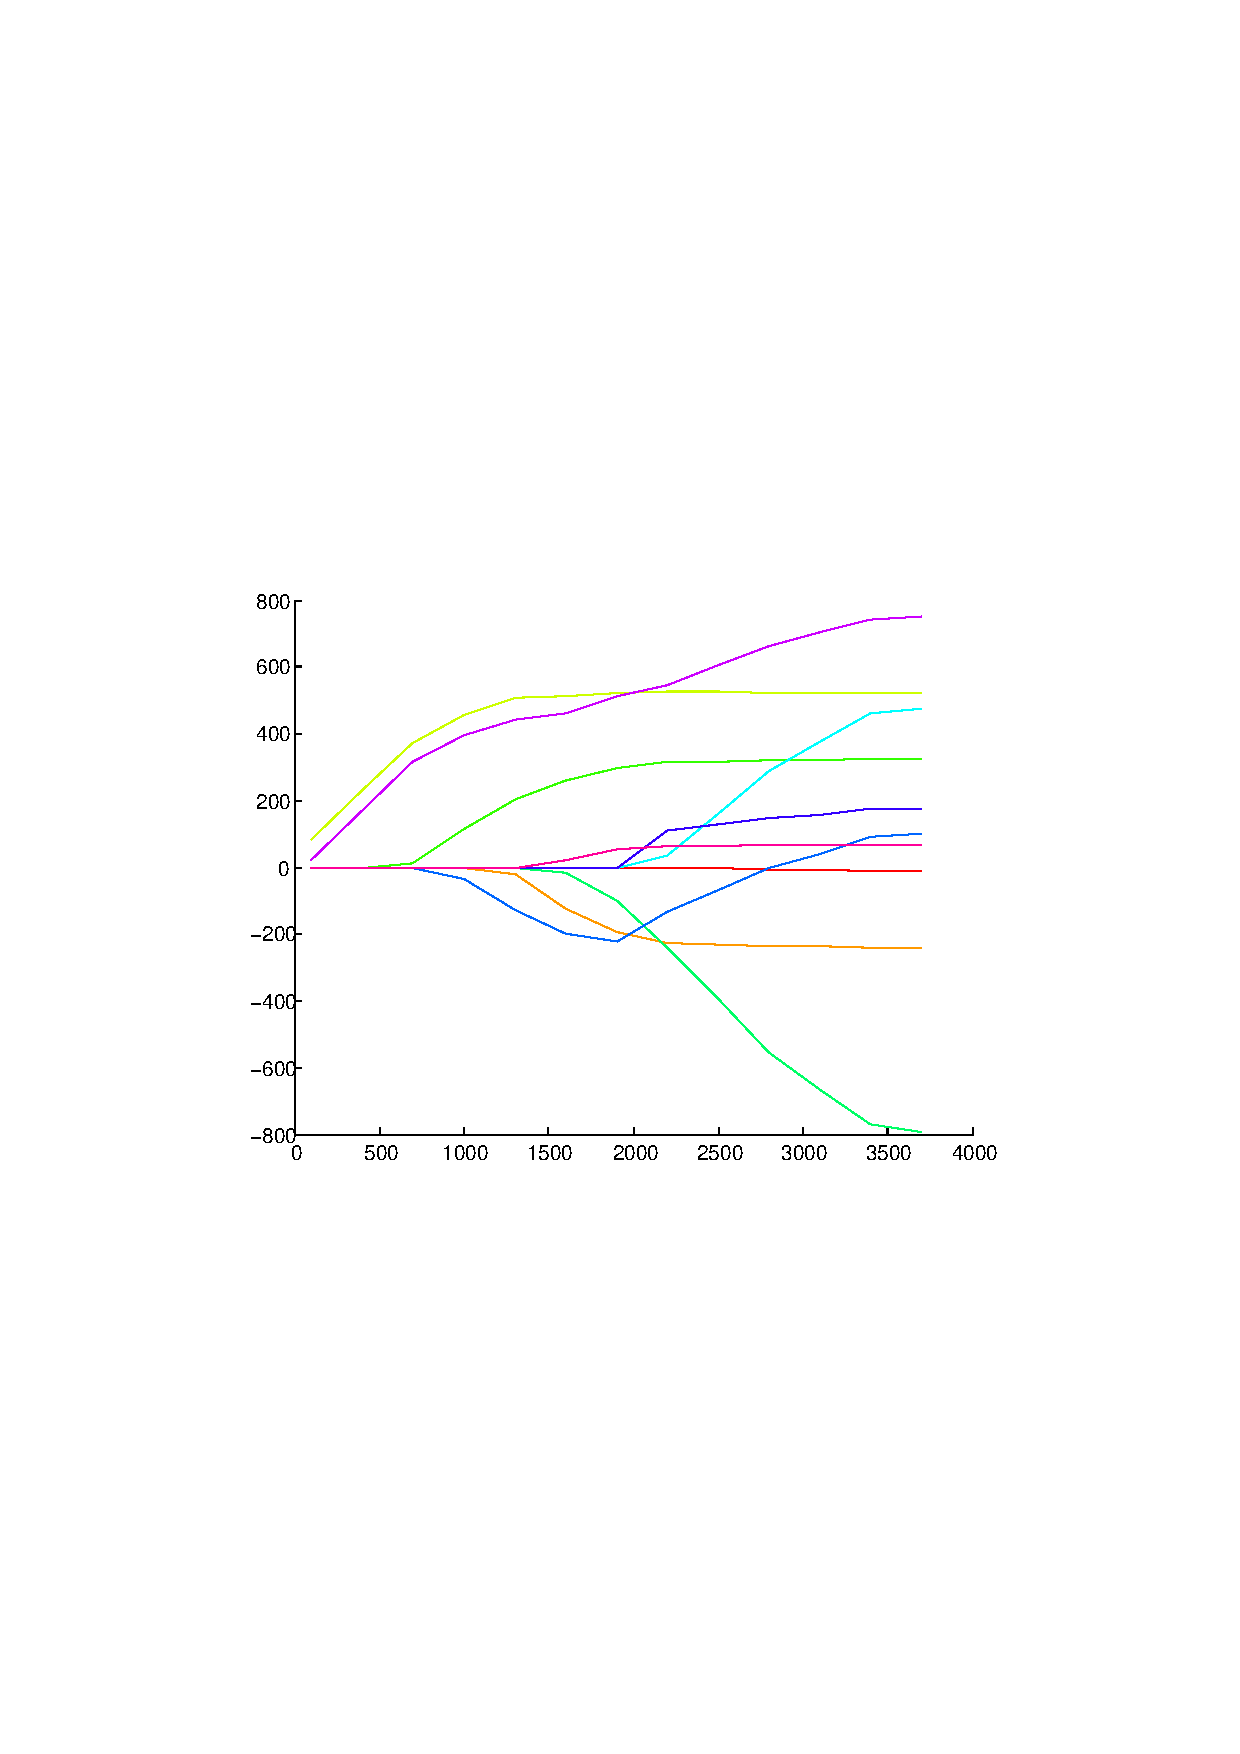
\includegraphics[width=\textwidth]{untitled.pdf}
	\caption{Estimates the regression coefficients $\beta_j, j = 1,2,\cdots,10$, for diabetes study, as a function of $t=\sum_j|\beta_j|$.}
\end{figure}
\clearpage

\subsubsection*{References}


\small{
[1] Tibshirani, R. (1996). {\it Regression shrinkage and selection via the lasso.}  J. Royal. Statist. Soc B., Vol. 58, No. 1, pages 267-288). 


[2] Busa J. (2012). {\it Solving quadratic programming problem with linear constraints containing absolute values[J]. } Acta Electrotechnica et Informatica,  12(3): 11-18.


[3] Efron B, Hastie T, Johnstone I, et al. (2004) {\it Least angle regression[J].} The Annals of statistics, 32(2): 407-499.

\end{document}
